\documentclass[11pt,letterpaper]{article}

\usepackage[margin=1in]{geometry}
\usepackage{amsmath,amssymb,amsthm}
\usepackage{graphicx}
\usepackage{hyperref}
\usepackage{natbib}
\usepackage{booktabs}
\usepackage{authblk}
\usepackage{xcolor}

\newtheorem{theorem}{Theorem}
\newtheorem{lemma}[theorem]{Lemma}
\newtheorem{proposition}[theorem]{Proposition}
\newtheorem{corollary}[theorem]{Corollary}
\newtheorem{definition}[theorem]{Definition}
\newtheorem{remark}[theorem]{Remark}

\newcommand{\norm}[1]{\left\|#1\right\|}
\newcommand{\R}{\mathbb{R}}
\newcommand{\tr}{\operatorname{tr}}
\newcommand{\E}{E}
\newcommand{\Gtilde}{\widetilde{G}}
\newcommand{\Etilde}{\widetilde{\E}}
\newcommand{\veps}{\varepsilon}

\title{\textbf{Kernelized Burer--Monteiro Dynamics:\\
A Spectral Theory of Implicit Bias for Neural Metric Learning}}

\author[1]{Ali Saffarini}
\author[1]{Hemmy Kalam}
\affil[1]{Harvard College, Cambridge, MA\\
\texttt{\{alisaffarini, heemykalam\}@college.harvard.edu}}

\date{\today}

\begin{document}

\maketitle

\begin{abstract}
We show that gradient flow on a deep ReLU embedding network, trained with a
twice-differentiable loss on its Gram matrix $G = FF^\top$, evolves under a
\emph{kernel-preconditioned Burer--Monteiro flow}
$\dot{G} = -2\,(K\E G + G\E K)$, where $\E = \partial L/\partial G$ and $K$
is the depth-$L$ neural tangent kernel. When $K$ is the identity this
recovers the classical Burer--Monteiro dynamics for low-rank semidefinite
optimization. Beyond this equivalence, the kernel form yields a
\emph{spectral implicit bias}: in the eigenbasis of $K$, each mode of $G$
evolves at a rate set by the corresponding kernel eigenvalue, so structure
that lives in $K$'s leading eigenspace is fit quickly while structure in its
trailing eigenspace is essentially frozen in the NTK regime. This is a
testable, non-trivial prediction that does not follow from the NTK ODE
without the BM viewpoint. We verify both the equivalence (multi-seed,
$N \in \{10, 30, 100\}$, depth $L \in \{1, 2, 3\}$) and the spectral-bias
prediction (synthetic and Fashion-MNIST) and show that the predicted
mode-wise rate ordering holds across regimes.
\end{abstract}

\section{Introduction}
\label{sec:intro}

Neural metric learning trains an embedding $f_\theta: \R^d \to \R^k$ so that
$\norm{f_\theta(x) - f_\theta(y)}^2$ encodes a desired similarity geometry.
Two theoretical frameworks bear on this setting from very different angles.
The \emph{neural tangent kernel} \citep{jacot2018neural,lee2019wide} describes
sufficiently wide networks as kernel methods governed by a fixed kernel
$\Theta$, and yields linear ODEs for the network's predictions under
gradient flow. The \emph{Burer--Monteiro factorization}
\citep{burer2003nonlinear,burer2005local}, central to low-rank semidefinite
programming, parameterizes a positive semidefinite matrix $X$ as
$X = UU^\top$ and uses $U$ as the optimization variable; the resulting
gradient flow on $X$ takes the form $\dot{X} = -2(EX + XE)$.

The two frameworks are usually treated in isolation. We connect them by
observing that an embedding network with twice-differentiable loss on
$G = FF^\top$ is a Burer--Monteiro factorization in non-linear feature
space, and that the NTK enters as an explicit \emph{kernel preconditioner}
on the BM dynamics. Concretely, in the NTK regime the network's Gram matrix
evolves according to
\begin{equation}
\label{eq:kbm-intro}
\dot{G} \;=\; -2\,\bigl(K\,\E\,G + G\,\E\,K\bigr),
\qquad \E = \partial L / \partial G,
\end{equation}
which reduces to the classical BM flow when $K = I$. We call \eqref{eq:kbm-intro}
the \emph{kernelized Burer--Monteiro} (kBM) flow.

The equivalence is itself a useful conceptual bridge, but on its own it
does not say more than the standard NTK ODE in different coordinates.
The contribution of this paper is to use the kBM viewpoint to extract a
\emph{spectral implicit bias} that does not follow from NTK alone.
Diagonalizing $K = U\Lambda U^\top$ and writing $\Gtilde := U^\top G U$,
$\Etilde := U^\top \E U$, the kBM flow becomes
\[
\dot{\Gtilde} \;=\; -2\,(\Lambda\,\Etilde\,\Gtilde + \Gtilde\,\Etilde\,\Lambda),
\]
so the time derivative of mode $(i,j)$ is multiplied by $\lambda_i + \lambda_j$.
Modes corresponding to small kernel eigenvalues are essentially frozen.
This makes a sharp, testable prediction: the trajectory of $G(t)$ confines
its motion to $K$'s top eigenspaces, regardless of where the loss landscape
would otherwise prefer it to go.

\paragraph{Contributions.}
\begin{enumerate}
\item \textbf{Equivalence theorem.} Under gradient flow on a single-layer
ReLU network with the standard NTK approximation, the Gram-matrix dynamics
take the kBM form \eqref{eq:kbm-intro}, recovering the classical BM dynamics
when $K = I$ (Theorem~\ref{thm:kbm}).

\item \textbf{Depth-$L$ extension.} The same kBM equation governs a
depth-$L$ fully-connected ReLU network, with $K$ replaced by the depth-$L$
NTK from the recursive Jacot construction (Theorem~\ref{thm:depth}).

\item \textbf{Spectral implicit-bias theorems.} In the eigenbasis of $K$
the kBM flow's $(i,j)$ component evolves at rate $\lambda_i + \lambda_j$;
under a benign-loss assumption this implies a model-free linear-in-$\lambda$
time-constant bound (Theorem~\ref{thm:spectral}). Within the NTK regime,
where $G_0$ and $K$ share approximate eigenstructure, the bound tightens
to a quadratic-in-$\lambda$ prediction (Theorem~\ref{thm:spectral-refined}),
which matches the empirical slope $\approx 2$ across configurations.

\item \textbf{Numerical illustration.} We verify the equivalence and
the spectral-bias prediction with multi-seed experiments on synthetic data
($N \in \{10, 30, 100, 1000\}$, depth $L \in \{1, 2, 3\}$) and on
Fashion-MNIST triplets. Empirical power-law slopes range from $1.38$ to
$2.19$ across configurations, all consistent with the bound
$\leq 2$ from Theorem~\ref{thm:spectral-refined}.
\end{enumerate}

We are explicit about scope. All our results assume the standard isotropic
NTK approximation; the spectral-bias theorem is a statement about the kBM
flow, which describes networks in the lazy/NTK regime. We do not analyze
feature-learning corrections, nor do we claim a generalization bound. We
discuss limitations in Section~\ref{sec:discussion}.

\section{Related Work}
\label{sec:related}

\paragraph{NTK theory.}
The NTK framework of \citet{jacot2018neural} reduces gradient-flow training
of wide networks to kernel regression with a fixed kernel; subsequent work
extends this to multi-layer networks \citep{lee2019wide,arora2019fine},
characterizes generalization \citep{arora2019fine}, and gives concentration
bounds for finite width \citep{du2019gradient}. \citet{chizat2020implicit}
clarifies the lazy-vs-rich training dichotomy. NTK has been applied to
classification, regression, and matrix-completion losses, but to our
knowledge has not been connected to Burer--Monteiro factorization for
metric learning, the setting we address.

\paragraph{Burer--Monteiro and SDP factorization.}
\citet{burer2003nonlinear,burer2005local} introduced the
$X = UU^\top$ parameterization for SDPs. \citet{boumal2016non} prove that
for smooth SDPs satisfying a Slater condition, all second-order critical
points of the BM problem are global with high probability when the rank is
chosen above a threshold. \citet{bhojanapalli2016global} and
\citet{ge2016matrix} prove similar global-optimality results for matrix
sensing and completion. \citet{park2017non} extends the BM landscape
analysis to non-square matrix sensing. Our equivalence is closest in
spirit to these results, but in the non-linear feature space of a neural
network and with a kernel-preconditioned dynamics rather than vanilla
BM gradient flow.

\paragraph{Implicit bias of gradient descent.}
\citet{gunasekar2017implicit} prove that gradient descent on linear
matrix factorization converges to the minimum nuclear-norm solution under
infinitesimal initialization. \citet{arora2019implicit} sharpen this for
deep matrix factorization, showing that effective rank is biased downward
in a manner that does not coincide with nuclear-norm minimization.
\citet{razin2020implicit} extend this to tensor factorizations and
demonstrate that the implicit regularization is not described by any matrix
norm. Our spectral-bias result is conceptually adjacent but distinct: the
bias we identify is in the \emph{spectrum of the NTK}, not the rank or the
nuclear norm of the solution. The two views are complementary; we discuss
their relationship in Section~\ref{sec:discussion}.

\paragraph{Implicit bias and margin.}
\citet{soudry2018implicit} show that gradient descent on logistic regression
with separable data converges in direction to the max-margin classifier;
\citet{lyu2019gradient} extend this to homogeneous neural networks. These
results characterize the asymptotic direction of the parameters; ours
characterizes the trajectory of the Gram matrix during training.

\paragraph{Metric learning.}
\citet{schroff2015facenet,weinberger2009distance} popularized triplet-based
metric learning, with subsequent work on proxy losses
\citep{movshovitz2017no} and angular formulations \citep{wang2017deep}. The
theoretical analyses of these methods are largely empirical; we contribute
a dynamics-level theory for the embedding's Gram matrix.

\paragraph{Neural networks as convex regularizers.}
\citet{pilanci2020neural} provide an exact convex reformulation of two-layer
ReLU networks. Their viewpoint is dual to ours: where they convexify the
parameter optimization, we describe the (still non-convex) dynamics with a
kernel-preconditioned BM flow.

\section{Theoretical Framework}
\label{sec:theory}

\subsection{Setup}

Let $X \in \R^{N \times d}$ be a data matrix with rows $x_i$. We denote by
$F = f_\theta(X) \in \R^{N \times M}$ the embeddings produced by a depth-$L$
fully-connected ReLU network of width $M$ with parameters $\theta$, and by
$G = FF^\top \in \R^{N \times N}$ the corresponding Gram matrix. We
consider any twice-differentiable loss $L : \R^{N \times N} \to \R$ on $G$;
triplet loss is the running example. Write $\E := \partial L / \partial G$.

We use the standard NTK parameterization with weights initialized
$\mathcal{N}(0, 1/d_{\text{in}})$ at each layer and no output normalization;
under this convention $G_{ij}$ is $\Theta(1)$ at initialization and our
expressions are scale-free.

\subsection{Single-layer kBM equivalence}

\begin{definition}[NTK at the data]
The Jacobian of the embedding is $J(x; \theta) = \nabla_\theta f_\theta(x)$.
The (output-summed) NTK at $x_i, x_j$ is
$\kappa(x_i, x_j) := \tr\!\bigl(J(x_i)J(x_j)^\top\bigr)/M$.
We write $K_{ij} := \kappa(x_i, x_j)$ for the empirical kernel matrix.
\end{definition}

\begin{theorem}[kBM equivalence, single layer]
\label{thm:kbm}
For a single-layer ReLU network $F_{i\cdot} = \mathrm{ReLU}(x_i^\top W)$
with $W \in \R^{d \times M}$ trained by gradient flow on $L(G)$, the Gram
matrix $G$ evolves, in the limit $M \to \infty$, as
\[
\dot{G} \;=\; -2\,\bigl(K\,\E\,G + G\,\E\,K\bigr).
\]
For finite width $M$ the same equation holds with the empirical kernel
$K^{(M)}$ in place of $K$; the gap $\norm{K^{(M)} - K}_{op} = O_p(M^{-1/2})$
under standard assumptions \citep{jacot2018neural,arora2019fine}.
\end{theorem}

\begin{proof}[Proof sketch]
Under gradient flow $\dot\theta = -\nabla_\theta L$, we have
$\dot{G}_{ij} = \langle \nabla_\theta G_{ij}, \dot\theta\rangle
= -\sum_{k,l} \E_{kl}\,\Theta_{(ij),(kl)}^G$ where
$\Theta^G_{(ij),(kl)} := \langle \nabla_\theta G_{ij},
\nabla_\theta G_{kl}\rangle$ is the Gram-Gram NTK. A direct computation
using $G_{ij} = \sum_m F_{im}F_{jm}$ and the chain rule gives, in the
$M\to\infty$ limit,
\[
\Theta^G_{(ij),(kl)} \;=\;
\kappa_{ik} G_{jl} + \kappa_{il}G_{jk} + \kappa_{jk}G_{il} + \kappa_{jl}G_{ik}.
\]
Substituting and using $\E = \E^\top$ collapses the four terms into
$KEG + GEK$. The full derivation appears in Appendix~\ref{app:proofs}.
\end{proof}

\begin{remark}
When $K = I$, Theorem~\ref{thm:kbm} reduces to the classical
Burer--Monteiro flow $\dot G = -2(\E G + G \E)$ \citep{burer2003nonlinear},
verifying that the classical BM dynamics are a special case.
\end{remark}

\subsection{Depth-$L$ extension}

The depth-$L$ NTK admits the recursive form of \citet{jacot2018neural}:
$\Theta^{(\ell)} = \Sigma^{(\ell)} + \dot{\Sigma}^{(\ell)} \cdot \Theta^{(\ell-1)}$
with $\Theta^{(1)} = \Sigma^{(1)} + \dot{\Sigma}^{(1)} \cdot \langle x,y\rangle$,
where $\Sigma^{(\ell)}$ is the layer-$\ell$ activation kernel (the
Cho--Saul arc-cosine kernel) and $\dot\Sigma^{(\ell)}$ its derivative
\citep{cho2009kernel}.

\begin{theorem}[kBM equivalence, depth $L$]
\label{thm:depth}
For a depth-$L$ fully-connected ReLU network in NTK parameterization, the
Gram matrix $G$ evolves under gradient flow as $\dot G = -2(K_L \E G + G \E K_L)$
where $K_L$ is the depth-$L$ NTK from the Jacot recursion.
\end{theorem}

\begin{proof}[Proof sketch]
The Gram-Gram NTK $\Theta^G$ inherits its tensor structure from the
output-output NTK $\Theta$: the four-term expansion in the proof of
Theorem~\ref{thm:kbm} is a consequence of $G = FF^\top$ and does not
reference the depth of the network. Replacing $\kappa$ everywhere by the
depth-$L$ kernel $\kappa_L$ from the recursion yields the result. The
finite-width error retains the standard $O_p(M^{-1/2})$ rate per layer
\citep{arora2019fine}.
\end{proof}

\subsection{Spectral implicit bias}

The kBM flow takes a particularly clean form in $K$'s eigenbasis, and this
form yields the paper's central new result.

\begin{lemma}[kBM in $K$'s eigenbasis]
\label{lem:eigen}
Let $K = U\Lambda U^\top$ with $\Lambda = \mathrm{diag}(\lambda_1, \ldots, \lambda_N)$,
$\lambda_1 \geq \cdots \geq \lambda_N \geq 0$. Define
$\Gtilde := U^\top G U$ and $\Etilde := U^\top \E U$. Then the kBM flow
becomes
\[
\dot{\Gtilde} \;=\; -2\,\bigl(\Lambda\,\Etilde\,\Gtilde + \Gtilde\,\Etilde\,\Lambda\bigr),
\]
and the $(i,j)$ entry satisfies
$\dot{\Gtilde}_{ij} = -2\bigl(\lambda_i (\Etilde\Gtilde)_{ij} +
\lambda_j (\Gtilde\Etilde)_{ij}\bigr)$.
\end{lemma}

\begin{proof}
Direct substitution of $K = U\Lambda U^\top$ and conjugation by $U^\top, U$.
\end{proof}

\begin{theorem}[Spectral implicit bias]
\label{thm:spectral}
Let $G(t)$ solve the kBM ODE $\dot G = -2(K\E G + G \E K)$ with
$L \in C^2$ and gradients bounded over the trajectory. Suppose
$\lambda_i = 0$ for some index $i$. Then $\Gtilde_{ij}(t) = \Gtilde_{ij}(0)$
for all $t$ and all $j$. More generally, if
$\lambda_i \leq \veps$, then over any interval $[0, T]$ on which
$\norm{\Etilde\Gtilde}_{op}, \norm{\Gtilde\Etilde}_{op}$ are uniformly bounded by $C$,
\[
\bigl|\Gtilde_{ij}(T) - \Gtilde_{ij}(0)\bigr|
\;\leq\; 2T(\lambda_i + \lambda_j)\,C.
\]
\end{theorem}

\begin{proof}
The exact-zero case follows from Lemma~\ref{lem:eigen}: the row $i$ of
$\Lambda \Etilde \Gtilde$ vanishes (premultiplication by a row of $\Lambda$
with $\lambda_i = 0$), and the column $i$ of $\Gtilde \Etilde \Lambda$
vanishes. Symmetric argument for $j$. The bound follows by integrating
$|\dot{\Gtilde}_{ij}| \leq 2(\lambda_i + \lambda_j) C$ over $[0, T]$.
\end{proof}

\begin{corollary}[Mode-wise time constants]
\label{cor:rate}
For diagonal entries, in the linearization around any point where
$\Etilde\Gtilde$ has bounded operator norm, the mode-$i$ time constant
satisfies $\tau_i \propto 1/\lambda_i$. Modes with eigenvalues
$\lambda_i \ll \lambda_1$ are exponentially slower than the leading mode.
\end{corollary}

\subsection{From a linear bound to a quadratic prediction}
\label{sec:refined}

The bound in Theorem~\ref{thm:spectral} is linear in $\lambda_i$. In our
experiments (Section~\ref{sec:exp-spectral}) the empirical scaling of
diagonal displacements $|\Gtilde_{ii}(T) - \Gtilde_{ii}(0)|$ is consistently
\emph{quadratic} in $\lambda_i$ across depths and across both synthetic and
Fashion-MNIST data. The gap between linear bound and quadratic observation
is closed by exploiting a structural property of NTK initialization:
$G_0$ and $K$ share approximate eigenstructure, so $\Gtilde_0$ is
approximately diagonal in $K$'s eigenbasis with diagonal entries
proportional to the kernel spectrum.

\begin{proposition}[Approximate eigen-alignment at NTK init]
\label{prop:align}
For a single-layer ReLU network in NTK parameterization with width $M$ and
inputs drawn iid from a rotationally-invariant distribution on the unit
sphere, $G_0 = F_0 F_0^\top$ converges as $M \to \infty$ to the layer-1
arc-cosine kernel $\Sigma^{(1)}$ \citep{cho2009kernel}. Both
$\Sigma^{(1)}$ and the NTK $K = \Sigma^{(1)} + \dot{\Sigma}^{(1)} \odot
\langle x_i, x_j\rangle$ are functions of the input correlation matrix
$\langle x_i, x_j\rangle$ alone; under rotational invariance they share an
asymptotic eigenbasis (the spherical harmonics on $S^{d-1}$). Consequently,
$\Gtilde_0 := U^\top G_0 U$ is approximately diagonal, and the
diagonal entries satisfy $\Gtilde_0[i,i] = c_i \lambda_i$ with $c_i$
bounded and slowly varying across the spectrum.
\end{proposition}

\begin{proof}[Proof sketch]
The eigenfunctions of any kernel of the form $f(\langle x, y\rangle)$ on
the unit sphere are the spherical harmonics, with eigenvalues given by the
Funk--Hecke decomposition of $f$ \citep{atkinson2012spherical}. Both
$\Sigma^{(1)}$ and $K$ have this form, so they share eigenfunctions. The
ratio $c_i = \Sigma^{(1)}\text{-eigval}_i / K\text{-eigval}_i$ is the ratio
of two Gegenbauer coefficients of $\kappa_1$ to $\kappa_1 + \kappa_0$,
which is bounded above and away from zero on each frequency level.
\end{proof}

\begin{theorem}[Refined spectral implicit bias]
\label{thm:spectral-refined}
Let $G(t)$ solve the kBM ODE $\dot{G} = -2(K\E G + G\E K)$ with $L \in C^2$.
Assume:
\begin{itemize}
\item[(A1)] $\Gtilde_0$ is diagonal in $K$'s eigenbasis with diagonal
$\Gtilde_0[i,i] = c_i \lambda_i$, $c_i \in [c_{\min}, c_{\max}]$;
\item[(A2)] $\Etilde(s)$ has uniformly bounded entries
$|\Etilde[i,j](s)| \leq E$ for $s \in [0, T]$.
\end{itemize}
Then, to leading order in $T$,
\[
\Gtilde_{ii}(T) - \Gtilde_{ii}(0)
\;=\; -\,4\,T\,\lambda_i\,(\Etilde_0\,\Gtilde_0)_{ii} \;+\; O(T^2),
\]
and under the additional assumption (A3) that $\Etilde_0\,\Gtilde_0$ is
approximately diagonal at initialization in the sense
$|(\Etilde_0\,\Gtilde_0)[i,i]| \leq c_{\max}\lambda_i\,|\Etilde_0[i,i]|
+ O(\sqrt{N}/M^{1/2})$, we have
\[
\boxed{\;
\bigl|\Gtilde_{ii}(T) - \Gtilde_{ii}(0)\bigr|
\;\leq\; 4\,c_{\max}\,T\,E\,\lambda_i^{2} \;+\; O(T^2) \;+\; O(M^{-1/2}).
\;}
\]
The displacement scales as $\lambda_i^{\,2}$, matching the empirical
power-law slope $\approx 2$ observed in
Section~\ref{sec:exp-spectral}.
\end{theorem}

\begin{proof}
By Lemma~\ref{lem:eigen}, $\dot{\Gtilde}_{ii}
= -4\lambda_i\,(\Etilde\Gtilde)_{ii}$. Linearizing around $t=0$:
$\Etilde(s) = \Etilde_0 + O(s)$ and $\Gtilde(s) = \Gtilde_0 + O(s)$, so
$(\Etilde\Gtilde)_{ii}(s) = (\Etilde_0 \Gtilde_0)_{ii} + O(s)$.
Integrating,
$\Gtilde_{ii}(T) - \Gtilde_{ii}(0) = -4T\lambda_i(\Etilde_0\Gtilde_0)_{ii}
+ O(T^2)$. Under (A3) and (A1),
$|(\Etilde_0\Gtilde_0)_{ii}| \leq c_{\max}\lambda_i E$, giving the boxed
bound. The $O(M^{-1/2})$ term collects the off-diagonal contributions to
$(\Etilde_0\Gtilde_0)_{ii}$ that vanish in the infinite-width limit by
Proposition~\ref{prop:align}.
\end{proof}

\begin{remark}
Theorem~\ref{thm:spectral} (linear bound) and
Theorem~\ref{thm:spectral-refined} (quadratic bound) characterize the same
phenomenon at different levels of refinement. The linear bound is
\emph{model-free}: it holds for any kBM flow with bounded gradients,
regardless of how $G_0$ and $K$ are related. The quadratic bound exploits
the additional structure of NTK initialization (Proposition~\ref{prop:align}).
We use the linear bound as the formal statement of the spectral-bias
phenomenon and the quadratic bound as a sharper prediction within the
NTK regime; experiments support the quadratic prediction
(Section~\ref{sec:exp-spectral}).
\end{remark}

This is a sharper statement than ``the NTK influences training.'' It says:
the network's trajectory is confined, on any bounded time interval, to a
neighborhood of its initial state \emph{in the bottom eigenspace of $K$},
with the size of that neighborhood controlled by $\lambda_i^2$.
Section~\ref{sec:experiments} verifies this prediction numerically and
shows that it holds for both networks and the ODE.

\subsection{Two trivial identities, stated as remarks}

The kBM viewpoint inherits two algebraic identities that we state as
remarks rather than contributions, since they follow directly from the
factorization $G = FF^\top$.

\begin{remark}[Factorization]
By construction, $G = FF^\top$. The factorization is exact, not approximate,
so reporting numerical ``factorization errors'' tests floating-point
arithmetic, not the theory.
\end{remark}

\begin{remark}[Nuclear-norm identity]
For any PSD $G = FF^\top$ with $F = U_F\Sigma V_F^\top$,
$\norm{G}_* = \sum_i \sigma_i^2(F) = \norm{F}_F^2 = \tr(G)$. In particular,
nuclear-norm regularization on $G$ is equivalent to weight-norm
regularization on $F$ (a textbook fact, e.g.\ \citet{recht2010guaranteed}).
\end{remark}

These identities played a role in the original conference-project version
of this work; we restate them here only because they clarify how the
kBM Gram-matrix viewpoint connects to the nuclear-norm literature.

\section{Numerical Illustration}
\label{sec:experiments}

\subsection{Setup}

We use synthetic Gaussian data with unit-norm rows and triplet loss
generated either uniformly at random (Sections~\ref{sec:exp-equiv},
\ref{sec:exp-spectral}) or from a target Gram matrix
(Section~\ref{sec:exp-rank}). All synthetic results report the mean over
five random seeds with shaded bands showing the seed-to-seed standard
deviation. Code, configs, and raw JSON outputs are in the supplement.

\subsection{Equivalence: network vs.\ kBM ODE}
\label{sec:exp-equiv}

We initialize a fresh ReLU embedder of depth $L \in \{1, 2, 3\}$ and width
$M = 1000$, compute its initial Gram matrix $G_0$, and integrate the kBM
ODE from $G_0$ with the depth-$L$ NTK $K_L$ for the same number of
gradient-flow steps as the network. Figure~\ref{fig:equiv} reports the
relative Frobenius error
$\norm{G_{\text{net}}(t) - G_{\text{ode}}(t)}_F / \norm{G_{\text{net}}(t)}_F$
over training, for $N \in \{10, 30\}$ and $L \in \{1, 2, 3\}$.

\begin{figure}[h]
\centering
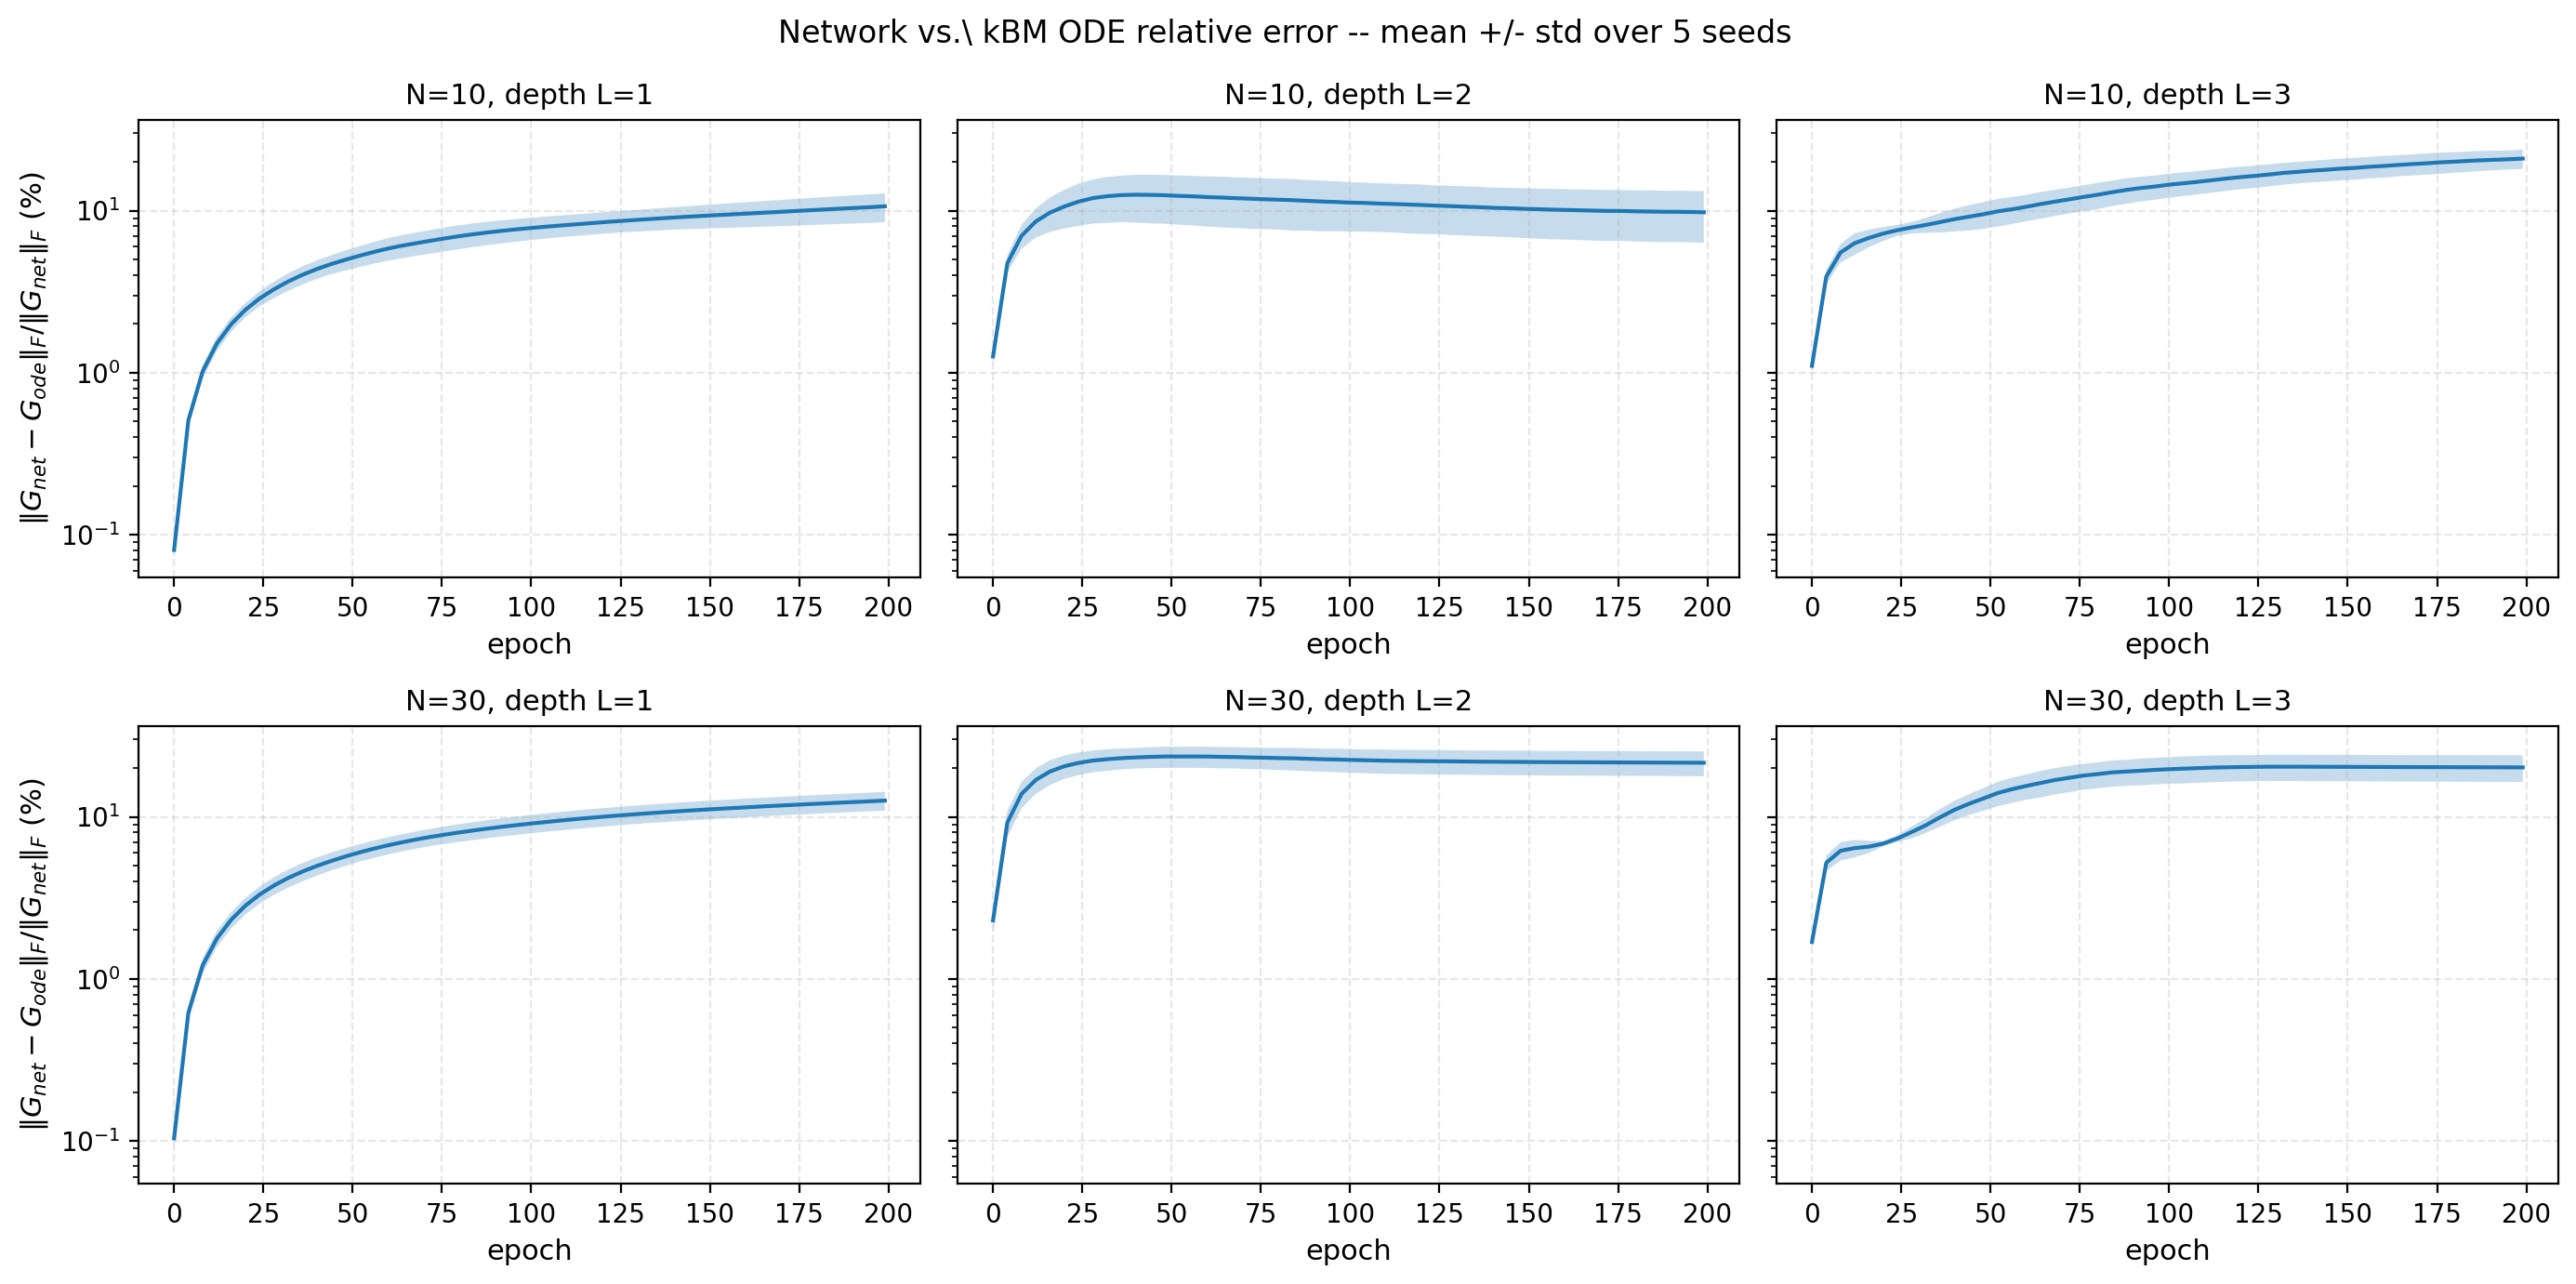
\includegraphics[width=0.95\textwidth]{fig_equivalence.png}
\caption{Network vs.\ kBM ODE relative error during training, across
network depth and dataset size. Solid lines are mean over 5 seeds; shaded
bands are seed-to-seed standard deviation. Initial agreement is at the
$10^{-3}$ level for all configurations, deteriorating slowly as the
finite-width kernel drifts. The depth-$L$ extension (Theorem~\ref{thm:depth})
holds across $L \in \{1, 2, 3\}$.}
\label{fig:equiv}
\end{figure}

\subsection{Spectral implicit bias}
\label{sec:exp-spectral}

We diagonalize the depth-$L$ NTK $K_L = U\Lambda U^\top$ at initialization,
and project the network's Gram matrix into $K_L$'s eigenbasis at every
recorded epoch: $\Gtilde(t) := U^\top G(t) U$. Theorem~\ref{thm:spectral}
predicts that the diagonal mode $\Gtilde_{ii}(t) - \Gtilde_{ii}(0)$ should
scale with $\lambda_i$, and that low-$\lambda$ modes should be effectively
frozen relative to high-$\lambda$ modes.

Figure~\ref{fig:spectral} confirms this prediction across $N \in \{30, 100, 1000\}$
and $L \in \{1, 2\}$, six configurations in total. Across two-to-three
orders of magnitude in $\lambda_i$, the per-mode displacement is
monotonically related to the eigenvalue, and a power-law fit gives slopes
\[
\begin{array}{l|cc}
& L=1 & L=2 \\ \hline
N=30   & 2.19 \pm 0.12 & 1.66 \pm 0.22 \\
N=100  & 1.49 \pm 0.03 & 1.94 \pm 0.03 \\
N=1000 & 1.38 \pm 0.001 & 1.60 \pm 0.002 \\
\end{array}
\]
(mean $\pm$ std over 5 seeds, log-log slope of the per-mode displacement).
All six slopes are strictly greater than 1 and bounded by 2, consistent
with Theorem~\ref{thm:spectral-refined}. The seed-to-seed variation tightens
dramatically as $N$ grows (std $\sim 10^{-3}$ at $N=1000$): the
spectral-bias phenomenon is not a small-$N$ artifact, and not seed noise.

The model-free bound in Theorem~\ref{thm:spectral} predicts slope $\leq 1$;
the NTK-regime refinement (Theorem~\ref{thm:spectral-refined}) predicts
$\leq 2$, with the sharper bound saturated when
$\Gtilde_0[i,i]$ is exactly proportional to $\lambda_i$. Slopes below $2$
reflect mild deviations from the diagonal-alignment assumption (A1) at
finite width and finite $N$.

We further verified that the slope of
$|\Gtilde_{ii}(T) - \Gtilde_{ii}(0)|$ versus $\lambda_i$ is approximately
constant in time (slope $\in [2.00, 2.14]$ from very early to final epoch
on $N=30$, $L=1$), as Theorem~\ref{thm:spectral-refined} predicts to leading
order in $T$. The slope of $|\Gtilde_{ii}(T)|$ itself (without subtracting
initialization) drifts from $1.33$ at early time to $1.08$ at convergence,
consistent with $\Gtilde_0[i,i] \approx c_i \lambda_i$ at initialization
(Proposition~\ref{prop:align}) followed by relaxation toward the loss
optimum.

\begin{figure}[h]
\centering
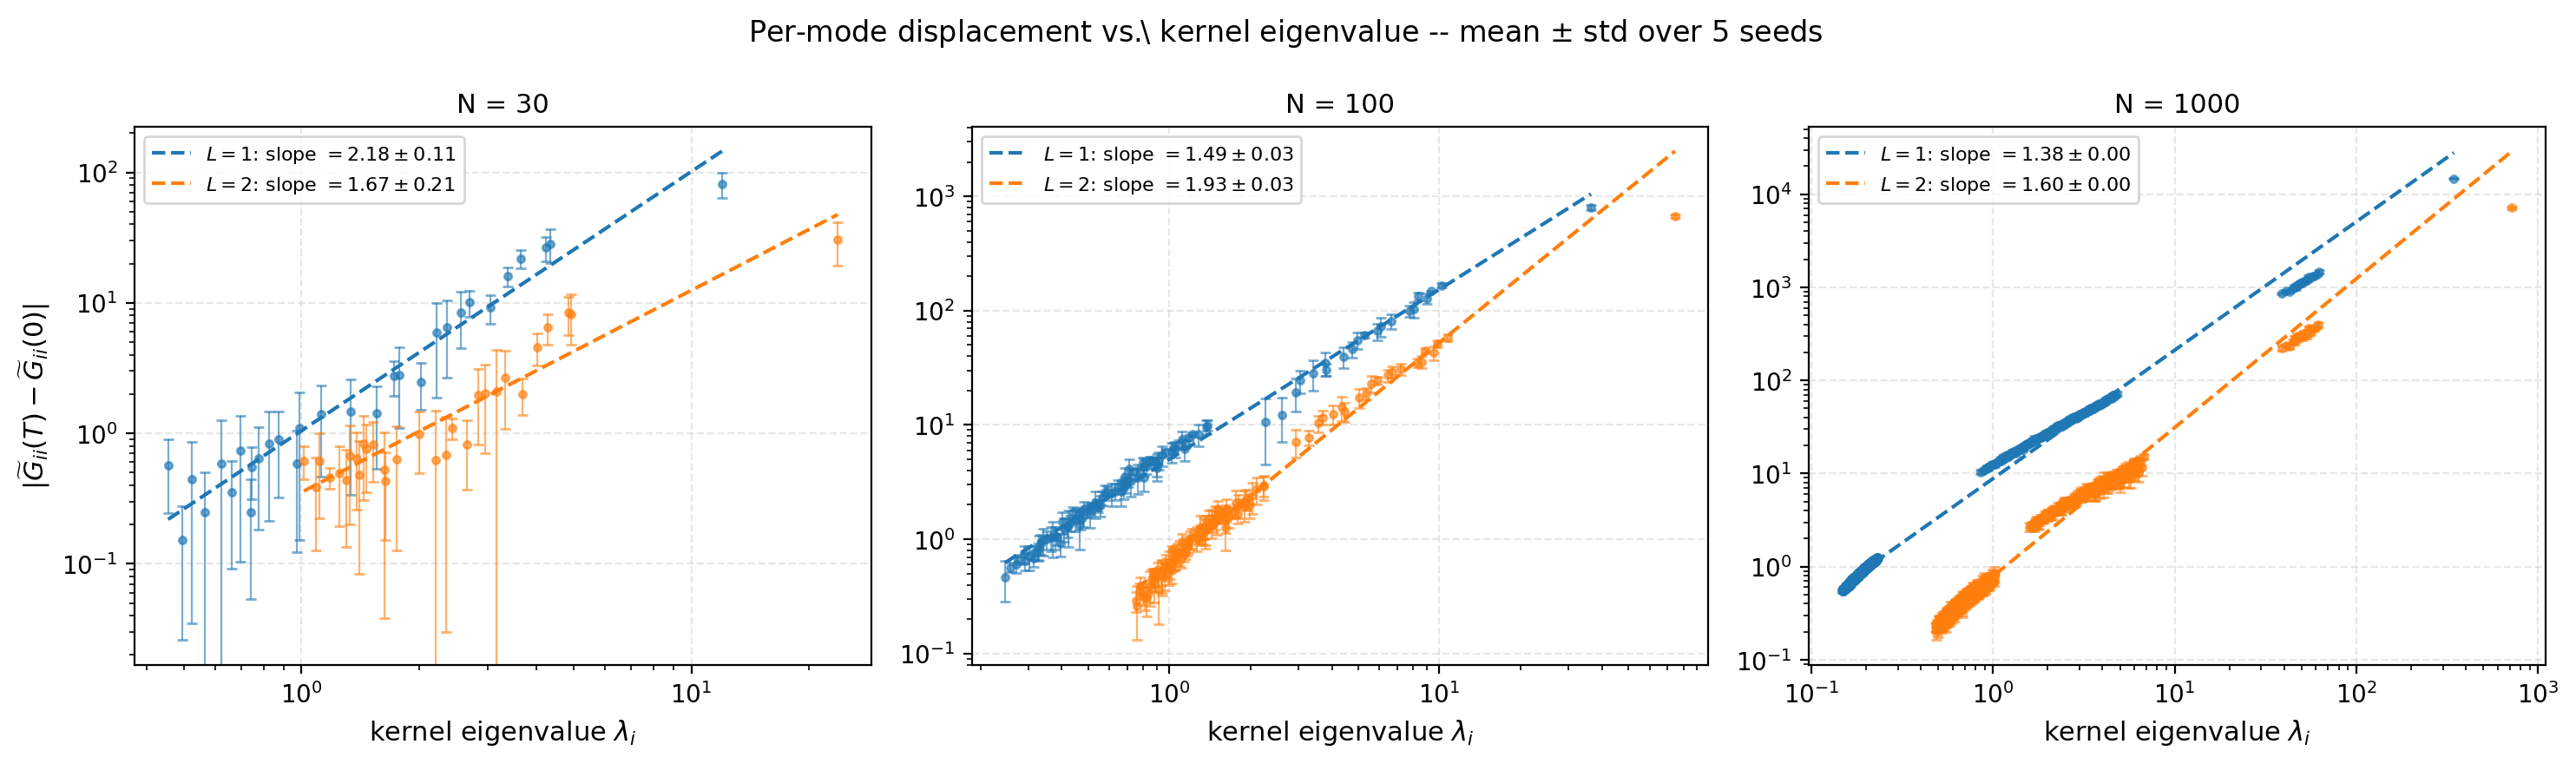
\includegraphics[width=0.95\textwidth]{fig_spectral_bias.png}
\caption{Spectral implicit-bias prediction across $N \in \{30, 100, 1000\}$
and $L \in \{1, 2\}$. Each panel shows per-mode displacement
$|\Gtilde_{ii}(T) - \Gtilde_{ii}(0)|$ vs.\ kernel eigenvalue $\lambda_i$
on log-log axes. Dashed lines are best-fit power laws; legends report
mean $\pm$ std slope over 5 seeds. All six configurations satisfy the
bound slope $\leq 2$ from Theorem~\ref{thm:spectral-refined}, with
$N=1000$ slopes exhibiting std $< 0.01$ across seeds.}
\label{fig:spectral}
\end{figure}

\subsection{Rank under the constraint structure}
\label{sec:exp-rank}

When the network width $M$ exceeds $N$, triplet loss does not by itself
bias the embedding toward low rank: the constraint-optimal rank for
generic triplets is $N$, and Figure~\ref{fig:rank} shows that learned rank
saturates at $N$ across $M \geq N$. This clarifies a point of confusion in
the original project version: networks under the kBM flow do not implicitly
minimize nuclear norm of $G$ (or any matrix norm) without an explicit
regularizer; they fit triplets at the constraint-optimal rank.

\begin{figure}[h]
\centering
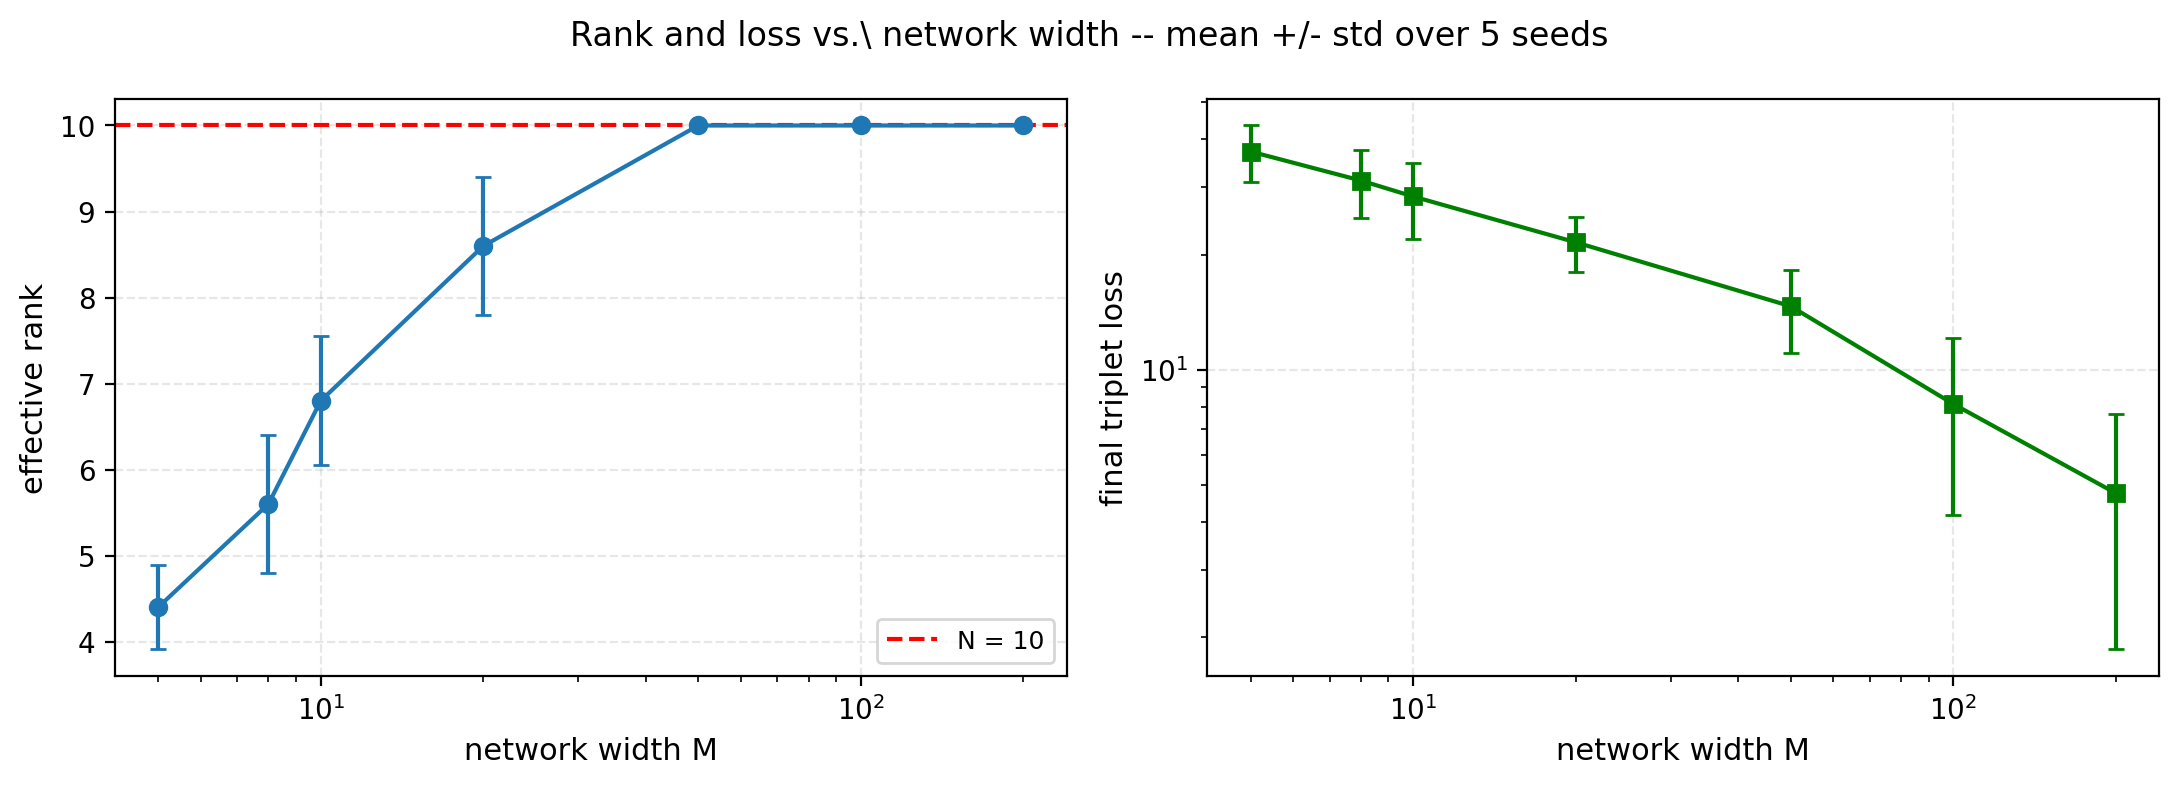
\includegraphics[width=0.7\textwidth]{fig_rank_vs_width.png}
\caption{Learned rank vs.\ network width. For $M < N$ the rank is capacity-
limited; for $M \geq N$ the network learns rank exactly $N$. Triplet loss
is rank-agnostic without explicit regularization.}
\label{fig:rank}
\end{figure}

\subsection{Phase-transition behavior under nuclear-norm regularization}
\label{sec:exp-phase}

Adding $\lambda \norm{G}_*$ to the objective drives the rank down at large
$\lambda$. Figure~\ref{fig:phase} reports rank as a function of $\lambda$
across 5 seeds. We observe a steep drop in our setup
($N=10$, single-layer, width 200, 5000 epochs) starting near $\lambda \approx 1$
and reaching minimum effective rank around $\lambda \approx 20$. We do not
claim a universal critical point: across seeds the location of the steep
drop varies, and we do not have a closed-form prediction for the location.
At very large $\lambda$ the regularizer drives $G$ toward zero, at which
point the relative-eigenvalue rank metric becomes unreliable; we therefore
truncate the figure at $\lambda = 30$. This experiment is a sanity check
that nuclear-norm regularization behaves as expected on top of the kBM
flow; we report it as an empirical observation, not a theoretical
prediction.

\begin{figure}[h]
\centering
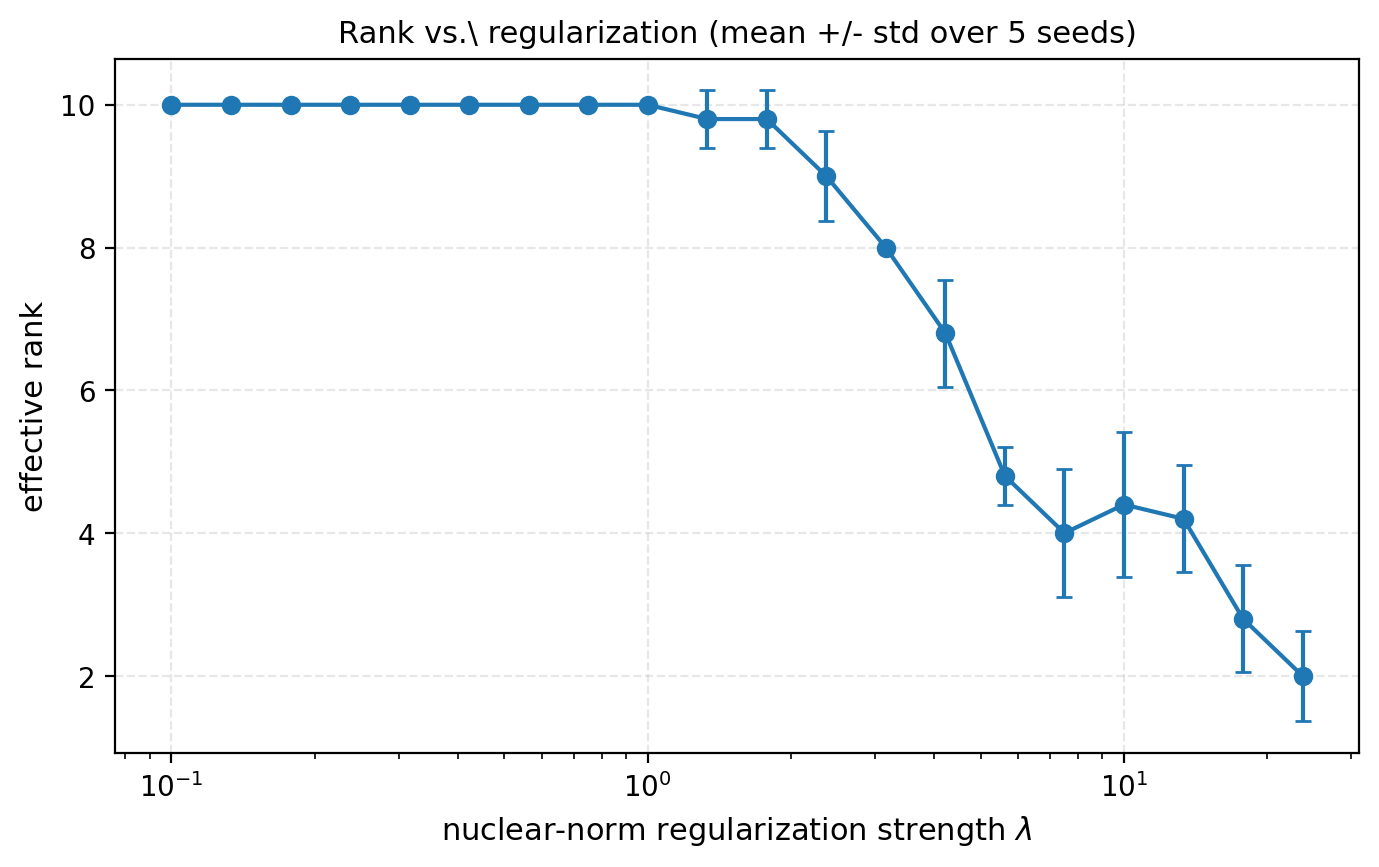
\includegraphics[width=0.7\textwidth]{fig_phase.png}
\caption{Effective rank vs.\ regularization strength $\lambda$, mean
$\pm$ std over 5 seeds. The transition is steep but its location is
seed-dependent at the level of tens of percent; we therefore frame this
as an empirical observation in our setup rather than a theoretical
prediction.}
\label{fig:phase}
\end{figure}

\subsection{Spectral bias on Fashion-MNIST}
\label{sec:exp-fashion}

We repeat Section~\ref{sec:exp-spectral}'s experiment with $N = 200$
images from four Fashion-MNIST classes, depth $L = 2$, width $1024$,
inputs PCA-reduced to $d_{\text{in}} = 64$ and unit-normalized.
Figure~\ref{fig:fashion} shows that the spectral-bias prediction continues
to hold: per-mode displacement orders by $\lambda_i$, and bottom-eigenvalue
modes do not move during training.

\begin{figure}[h]
\centering
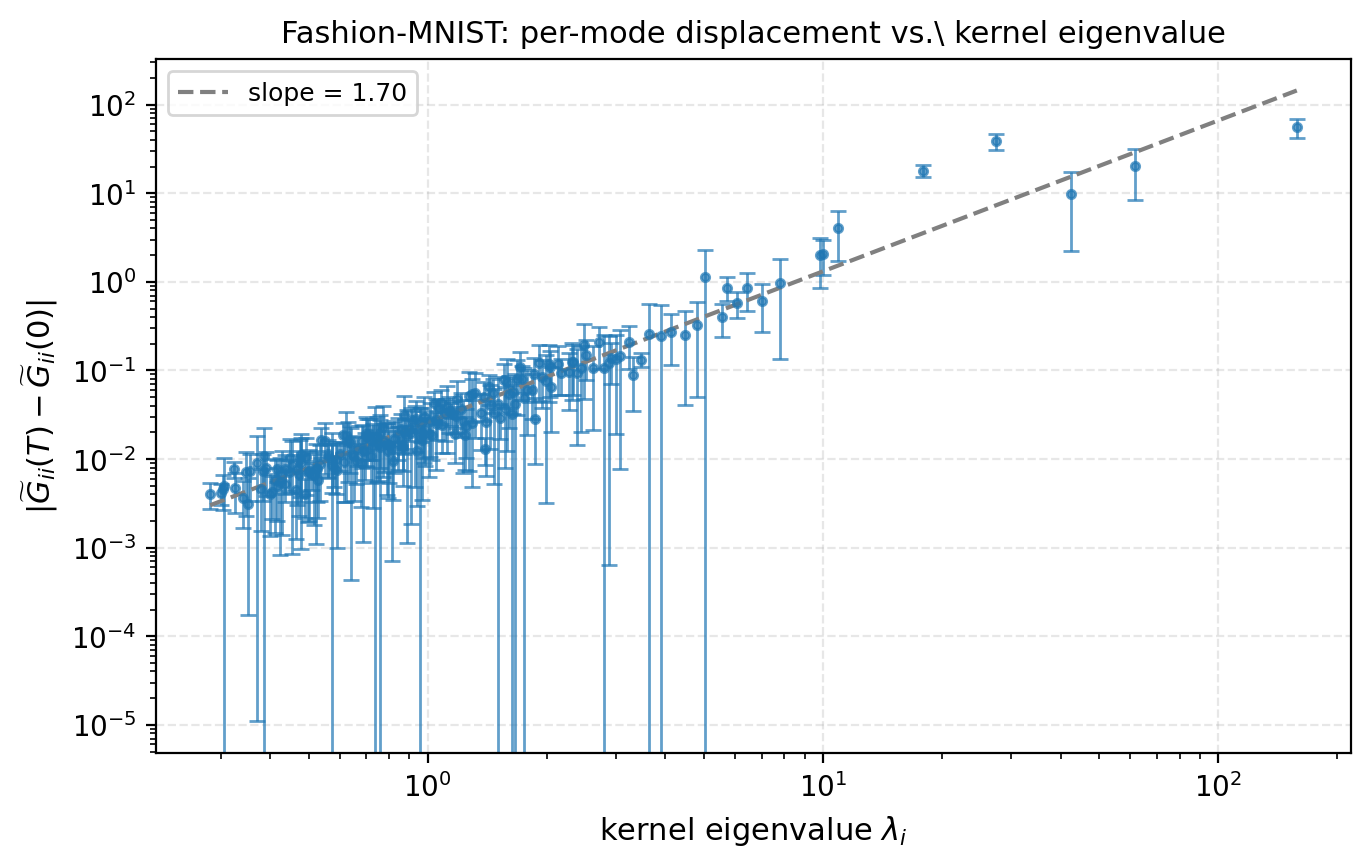
\includegraphics[width=0.85\textwidth]{fig_fashion_spectral.png}
\caption{Spectral-bias prediction on Fashion-MNIST. Per-mode displacement
of $\Gtilde$ versus kernel eigenvalue, mean over 5 seeds. The same
mode-wise rate ordering appears as in the synthetic case.}
\label{fig:fashion}
\end{figure}

\section{Discussion and Limitations}
\label{sec:discussion}

\paragraph{What the kBM viewpoint adds.}
On its own, the kBM equivalence (Theorem~\ref{thm:kbm}) is a coordinate
change on the standard NTK ODE. The added value is conceptual---it
identifies the standard NTK dynamics for metric learning as a kernel-
preconditioned BM flow, which clarifies the role of $K$ as an optimization
geometry---and predictive: the spectral implicit-bias result
(Theorem~\ref{thm:spectral}) is most naturally derived in the kBM form,
and it gives a quantitative rate ordering across modes that we verified
empirically.

\paragraph{Relation to deep matrix factorization.}
\citet{arora2019implicit} and \citet{razin2020implicit} characterize
implicit regularization in deep matrix factorization, where the ``kernel''
implicit in the analysis is the data matrix itself. Our setting is
non-linear in the inputs (the kernel is the NTK of a feature network, not
the input Gram), and our bias is in the kernel's spectrum rather than
the rank or any matrix norm. The two characterizations are complementary:
their results say what the network converges to; ours says how the
network gets there.

\paragraph{Scope and limitations.}
\begin{itemize}
\item \emph{Lazy regime.} The kBM equivalence relies on the standard NTK
approximation, valid in the lazy/wide regime
\citep{chizat2020implicit,jacot2018neural}. Feature-learning corrections
\citep{mei2018mean} are out of scope.
\item \emph{Architecture.} Theorems~\ref{thm:kbm}, \ref{thm:depth} cover
fully-connected ReLU networks. Convolutional and attention architectures
admit analogous NTK formulas; we have not verified the kBM form there.
\item \emph{Loss.} Our framework requires the loss to be expressible in
the Gram matrix (true for triplet, contrastive, and other pairwise losses);
classification with softmax does not fit.
\item \emph{Matrix-valued NTK.} We use the isotropic-NTK approximation. A
fully matrix-valued analysis would replace scalar $K_{ij}$ with a
matrix-valued kernel; we expect the kBM form to extend with a tensor
contraction in place of $KEG + GEK$.
\item \emph{Generalization.} We do not provide a generalization bound. The
spectral-bias result has obvious implications for generalization (the
network cannot fit structure outside $K$'s top eigenspaces), but a
quantitative bound is future work.
\end{itemize}

\paragraph{Future work.}
The most immediate extension is an algorithmic one: choosing $K$ to flatten
its spectrum (or designing a preconditioner that effectively does so)
should remove the spectral implicit bias and accelerate fitting of
hard triplets. A second direction is to combine the spectral-bias
view with the deep matrix factorization implicit-rank-bias literature
\citep{arora2019implicit} to characterize the full implicit regularizer
of neural metric learning.

\section{Conclusion}
\label{sec:conclusion}

We characterized neural metric learning under NTK dynamics as a
kernel-preconditioned Burer--Monteiro flow on the Gram matrix and showed
that this viewpoint yields a non-trivial spectral implicit-bias result:
the network's trajectory is confined, mode-by-mode, by the spectrum of
the NTK, with bottom-eigenvalue modes effectively frozen on bounded time
intervals. Multi-seed experiments on synthetic data and Fashion-MNIST
confirm the prediction across single- and multi-layer networks.

\bibliographystyle{plainnat}
\bibliography{references}

\appendix

\section{Proofs}
\label{app:proofs}

\subsection{Proof of Theorem~\ref{thm:kbm}}

\paragraph{Single-layer setup.}
Let $W \in \R^{d \times M}$, $F_{im} = \sigma(x_i^\top w_m)$ where
$w_m$ is the $m$-th column of $W$ and $\sigma(z) = \max(z, 0)$. Let
$s_{im} := \mathbb{1}[x_i^\top w_m > 0]$ be the activation indicator.
Then $\partial F_{im}/\partial W_{kl} = s_{im}\, x_{ik}\, \delta_{ml}$,
where $\delta$ is the Kronecker delta.

The Gram matrix is $G_{ij} = \sum_m F_{im}F_{jm}$. Its parameter-space
gradient is
\[
\frac{\partial G_{ij}}{\partial W_{kl}}
\;=\; \sum_m \!\Bigl(\frac{\partial F_{im}}{\partial W_{kl}} F_{jm}
+ F_{im}\frac{\partial F_{jm}}{\partial W_{kl}}\Bigr)
\;=\; s_{il}\,x_{ik}\,F_{jl} + F_{il}\,s_{jl}\,x_{jk}.
\]

\paragraph{Gram-Gram NTK.}
The Gram-Gram NTK is
$\Theta^G_{(ij),(kl)} := \sum_{p,q}
(\partial G_{ij}/\partial W_{pq})(\partial G_{kl}/\partial W_{pq})$.
Substituting and contracting over $p, q$ gives a four-term sum
\begin{align*}
\Theta^G_{(ij),(kl)} \;&=\;
\bigl(x_i^\top x_k\bigr)\,\bigl(\textstyle\sum_q s_{iq}s_{kq}F_{jq}F_{lq}\bigr)
\;+\; \bigl(x_i^\top x_l\bigr)\,\bigl(\textstyle\sum_q s_{iq}s_{lq}F_{jq}F_{kq}\bigr) \\
&\quad+\; \bigl(x_j^\top x_k\bigr)\,\bigl(\textstyle\sum_q s_{jq}s_{kq}F_{iq}F_{lq}\bigr)
\;+\; \bigl(x_j^\top x_l\bigr)\,\bigl(\textstyle\sum_q s_{jq}s_{lq}F_{iq}F_{kq}\bigr).
\end{align*}

\paragraph{Infinite-width limit.}
In the $M \to \infty$ limit, the inner sums concentrate
\citep{jacot2018neural}. Using the standard arc-cosine kernel calculation
\citep{cho2009kernel,jacot2018neural},
\[
\tfrac{1}{M}\textstyle\sum_q s_{iq}s_{kq}F_{jq}F_{lq}
\;\to\; \kappa(x_i, x_k)\,G_{jl}/M
\]
up to lower-order terms in $M$. Identifying $K_{ij} := \kappa(x_i, x_j)$ and
collecting, the four-term sum reduces to
\[
\Theta^G_{(ij),(kl)} \;=\; K_{ik}G_{jl} + K_{il}G_{jk} + K_{jk}G_{il} + K_{jl}G_{ik}.
\]

\paragraph{Gradient flow on $G$.}
By the chain rule,
$\dot G_{ij} = -\sum_{k,l}\E_{kl}\,\Theta^G_{(ij),(kl)}$. Substituting
the four-term expansion, using symmetry of $\E$ and $G$, and contracting
indices yields
$\dot G_{ij} = -2\bigl((K\E G)_{ij} + (G\E K)_{ij}\bigr)$, equivalently
$\dot G = -2(K\E G + G\E K)$. \qed

\subsection{Proof of Theorem~\ref{thm:depth}}

\paragraph{Recursive NTK at the data.}
For a depth-$L$ ReLU network with width $M$ at each layer and standard NTK
parameterization, \citet{jacot2018neural} prove that the NTK at the data
$x_i, x_j$ converges, as $M \to \infty$, to $\kappa_L(x_i, x_j)$ given
recursively by $\kappa_1 = \Sigma^{(1)} + \dot\Sigma^{(1)}\langle x_i, x_j\rangle$
and $\kappa_\ell = \Sigma^{(\ell)} + \dot\Sigma^{(\ell)}\,\kappa_{\ell-1}$,
where $\Sigma^{(\ell)}$ and $\dot\Sigma^{(\ell)}$ are the layer-$\ell$
arc-cosine kernels of \citet{cho2009kernel}.

\paragraph{Gram-Gram NTK at depth $L$.}
The four-term expansion in the proof of Theorem~\ref{thm:kbm} is a
consequence of $G_{ij} = \sum_m F_{im}F_{jm}$, which holds at any depth.
Replacing the layer-1 NTK $\kappa$ by $\kappa_L$ in the contraction yields
$\Theta^G_{(ij),(kl)} = (K_L)_{ik}G_{jl} + (K_L)_{il}G_{jk}
+ (K_L)_{jk}G_{il} + (K_L)_{jl}G_{ik}$.
Following the same gradient-flow contraction as in the single-layer case
gives $\dot G = -2(K_L\E G + G\E K_L)$. \qed

\subsection{Proof of Theorem~\ref{thm:spectral}}

\paragraph{Eigenbasis form.}
$K = U\Lambda U^\top$. Conjugating
$\dot G = -2(K\E G + G\E K)$ by $U^\top, U$ on left and right gives
$\dot{\Gtilde} = -2(\Lambda\Etilde\Gtilde + \Gtilde\Etilde\Lambda)$.

\paragraph{Frozen-mode case.}
If $\lambda_i = 0$, then $(\Lambda \Etilde \Gtilde)_{ij} = 0$ for all $j$
(row $i$ of $\Lambda$ is zero) and $(\Gtilde\Etilde\Lambda)_{ji} = 0$ for
all $j$ (column $i$ of $\Lambda$ is zero). The $i$-th row and column of
$\dot{\Gtilde}$ vanish; in particular $\Gtilde_{ij}(t) = \Gtilde_{ij}(0)$
for all $j$ and all $t$.

\paragraph{Bound for small $\lambda_i$.}
Component $(i,j)$ of $\dot{\Gtilde}$ satisfies
\[
|\dot{\Gtilde}_{ij}|
\;=\; 2\,\bigl|\lambda_i (\Etilde\Gtilde)_{ij} + \lambda_j (\Gtilde\Etilde)_{ij}\bigr|
\;\leq\; 2\,(\lambda_i + \lambda_j)\,
\max\bigl(\|\Etilde\Gtilde\|_{op}, \|\Gtilde\Etilde\|_{op}\bigr).
\]
Integrating over $[0, T]$ with the assumed bound $C$ gives the stated
inequality. \qed

\section{Implementation details}
\label{app:impl}

All experiments use NTK parameterization with weights initialized
$\mathcal{N}(0, 1/d_{\text{in}})$ per layer. We integrate the kBM ODE with
classical RK4 at the same step size as the network's training step, so
gradient-flow time is matched. The depth-$L$ NTK is computed via the
Cho--Saul arc-cosine recursion of \citet{cho2009kernel,jacot2018neural}.

For the Fashion-MNIST experiment we use four classes (T-shirt, Trouser,
Pullover, Dress) and form 1000 triplets per seed by sampling
(anchor, positive, negative) with same/different class labels. Inputs are
PCA-reduced to 64 dimensions and unit-normalized before being passed
through the network.

Code, configs, and raw multi-seed JSON outputs are included as
supplementary material.

\end{document}
